%%%%%%%%%%%%%%%%%%%%%%%%%%%%%%%%%%%%%%%%%%%%%%%%%%%%%%%%%%%%%%%%%%%%%%%%%
%           Capítulo 3: MARCO TEÓRICO - REVISIÓN DE LITERATURA
%%%%%%%%%%%%%%%%%%%%%%%%%%%%%%%%%%%%%%%%%%%%%%%%%%%%%%%%%%%%%%%%%%%%%%%%%

\chapter{Abandono de clientes.}

En este capítulo abordaremos el concepto de abandono de clientes, al ser este uno de los fenómenos que deseamos analizar y predecir, es de suma importancia comprender el concepto de abandono, esto para tener completo entendimiento sobre el comportamiento de los clientes y el fuerte impacto que puede tener el conocer el abandono dentro de una organización. En adelante nos referiremos al abandono como \textit{churn} y a la tasa de abandono como \textit{churn rate}.

La forma que usaremos para calcular la tasa de abandono en este trabajo sera la dada por \ref{EquationChurn}, como podemos apreciar esta expresión considera cierto enfoque temporal, más adelante abordaremos el porque.

\begin{equation}
	\textrm{Churn Rate}=\frac{\textrm{Número de clientes en el ultimo periodo}}{\textrm{Total de clientes}} -1 
	\label{EquationChurn}
\end{equation}

De hecho si tomamos la razon entre el numero de clientes en el ultimo periodo o en el actual y el total de clientes tendremos la tasa de retención de clientes. Entendiendo que la tasa de retención es el complemento de la tasa de abandono.
 
\section{Definición de \textit{churn}}

De hecho \citet[p. 36]{2020Gold} define el origen de la palabra \textit{churn} en el término \textit{churn rate}, este termino hace referencia a la proporción de clientes que abandonan la empresa en un periodo determinado. 

Más en especifico el \textit{churn} es un estado u estatus que se le da a un cliente habitual de una empresa o servicio cuando este da por terminada la relación comercial, este concepto ha sido acuñado más recientemente por aquellas empresas que prestan servicios de suscripciones, como pueden ser plataformas de entretenimiento digital, proveedores de servicios de telecomunicaciones (internet, telefonía y/o televisión), etc. Sin embargo el \textit{churn} no es únicamente aplicable a este tipo de compañías.

Ya que solo necesitamos que la empresa en cuestión oferte uno o más productos de los cuales tenga consumidores habituales para poder estudiar el \textit{churn} en toda su cartera de clientes y más en especifico poder abordar distintas estrategias para la retención de clientes. 

En general el estudiar el comportamiento de los clientes puede ser un reto distinto dependiendo de la empresa e industria en la cual el científico de datos o analista de datos se encuentre, por lo cual es necesario tener pleno conocimiento sobre las reglas de negocio en cuestión. Ya que cada caso de estudio necesitará de enfoques distintos para poder entender de mejor manera el \textit{churn} y cómo combatirlo.

De hecho ese debería ser el propósito principal de estudiar el \textit{churn}, poder proporcionar una radiografía certera sobre el comportamiento de los clientes en una empresa, esto eventualmente permitirá a los líderes dentro de la organización poder tomar decisiones basadas en datos, y es tarea del científico de datos proveer la información lo más clara y precisa posible.

\section{Metricas y causalidad del \textit{churn}}

Pese a que existen numerosas estrategias que podrían ayudar a disminuir la tasa de abandono y por lo tanto combatirlo, cabe resaltar que no nos enfocaremos en explicar dichas estrategias, más bien, nos enfocaremos en como aprovechar las razones subyacentes al \textit{churn} para poder definir buenas métricas \footnote{En este caso cabe aclarar que otros sinónimos con los nos referiremos a las metricas son características, dimensiones o variables predicadoras.} que ayuden a evaluar el comportamiento de los clientes, y así poder usar estas mismas métricas en una eventual predicción del \textit{churn}, el cual es propósito final de este trabajo.

Una definición de métrica para clientes puede ser la provista por \citet[p. 51]{2020Gold} ``\textit{cualquier medición que realice sobre todos los clientes individualmente}". Por lo cual es crucial encontrar las mejores metricas para monitorear a los clientes, de hecho \cite{2020Gold} menciona las siguientes características importantes que debe tener una buena métrica; debe ser fácil de entender para la empresa, deben estar asociada con el \textit{churn} y la retención, segmenta a los clientes de manera que facilita las intervenciones dirigidas a disminuir el \textit{churn rate} y sobre todo es útil para múltiples áreas de la empresa (marketing, soporte, etc.)

En el capitulo anterior discutimos sobre la importancia de seleccionar correctamente las características para implementar \textsl{modelos de clasificación binaria}, mencionamos diversas técnicas de reducción de dimensiones basadas en criterios estadísticos, sin embargo, hay que considerar otras pautas a la hora de escoger dichas dimensiones si lo que deseamos es predecir el \textit{churn}, estos juicios alternativos obedecen más a las reglas del negocio o empresa. Claro siempre hay que analizar la relación que pudieran tener con el \textit{churn}. 



\section{Como calcular el \textit{churn}}

Anteriormente expusimos la diversidad de enfoques del \textit{churn}, que hay empresas dedicadas a ofertar servicios de suscripciones o que simplemente tienen una cartera de clientes habituales, pese a todo esto no todas las empresas tienen un indicador de abandono, de hecho en la mayoría de los casos lo primero sea determinar de manera correcta cuando un cliente a abandonado.

Para ellos en nuestro conjunto de datos asignaremos como \textit{churn} a una columna cuyos registro sea true o false, esta fungirá como una bandera de abandono donde el valor true indica que un cliente abandono y False el caso contrario, como construir esta columna sera parte importante de este trabajo.

En el caso de las empresas que ofrecen suscripciones puede no aplicar, ya que saber cuando un cliente ha abandonado la compañía es más sencillo, podemos simplemente asignar el valor de True en la columna \textit{churn} a todos aquellos que no cuentan con una suscripción activa y como False a los casos contrarios, y como mencionamos anteriormente, hablaremos da como construir el indicador de \textit{churn}, para usar esta forma de determinar el \textit{churn} es necesario contar con una variable que nos indique el tiempo desde la ultima transacción del cliente, y aun que no contemos con este dato podríamos determinarlo fácilmente de la siguiente manera:

\begin{lstlisting}[language=Python, caption=Ejemplo del calculo de fecha desde la ultima compra, label=EjemplodeTDUC]
	fecha_ref = pd.Timestamp(datetime.now().date())
	df['Tiempo_ultima_compra'] = df.groupby('bp_id')['Date_Last'].transform(lambda x: np.abs((fecha_ref - x.max()).days))
	
\end{lstlisting}


Donde '$fecha\_ref$' es la variable que almacena la fecha del sistema cuando se ejecuta el programa, otra alternativa sería asignar a '$fecha\_ref$' un día en especifico, ejemplo el fin de mes. Por otra parte necesitamos una columna auxiliar en nuestro dataframe para realizar el calculo final que es el tiempo desde la ultima compra, esta columna es '$Date\_Last$', esta contiene la ultima fecha de compra del cada cliente y en base a esta calcularemos el tiempo trascurrido desde la ultima compra, tal y como se muestra en el código \ref{EjemplodeTDUC}.

Una vez determinada la columna $'Tiempo\_ultima\_compra'$ conviene analizar la distribución de los valores para dicha variable, esto nos permite ver el comportamiento general de cada individuo\footnote{En el capitulo 2 repasamos el análisis univariado y sus implicaciones teóricas, en esta sección nos enfocaremos unicamente en las aplicaciones.}, en este caso, podemos visualizar el histograma de la variable en cuestión (figura \ref{fig:enter-label5}) en la cual podemos apreciar que gran parte de los clientes no sobrepasan los 125 días de inactividad de compra, y de hecho podemos notar una linea vertical de color roja que indica el percentil 75 \footnote{Para este ejemplo, decidí tomar el percentil 75, sin embargo la elección de percentil es a criterio del científico de datos y esta fuertemente ligado a las caracteristicas de los datos con los que estemos trabajando, así que tómese este valor como lo que es, un ejemplo.} de la variable '$Tiempo\_ultima\_compra$' lo cual nos indica que los clientes con un tiempo de inactividad demasiado alto son realmente pocos.

\begin{center}
	\begin{figure}[H]
		\centering
		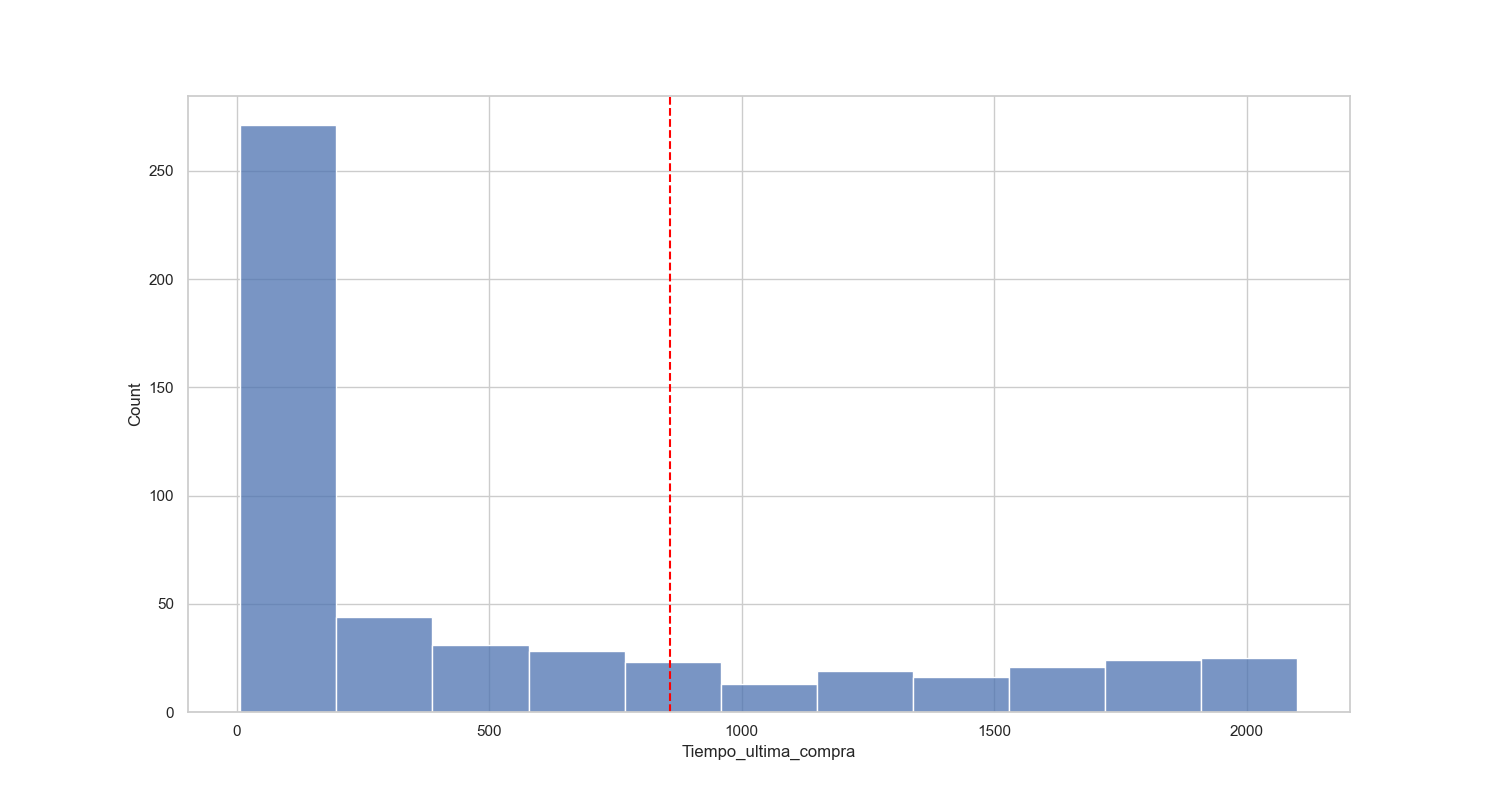
\includegraphics[scale=.35]{Gráficas e Imagenes/Tiempo_ultima_compra.png}
		\caption{Histograma de Tiempo desde la ultima compra}
		\label{fig:enter-label5}
	\end{figure}
\end{center}

Como sugerencia, conviene que incluyamos una columna en nuestro dataframe que contenga el percentil que deseamos tomar como condición para determinar el abandono, puedes seguir el ejemplo que se muestra en el código \ref{CalculoPercentil} como ejemplo de como realizar el calculo del k-esimo\footnote{Donde k es el valor del percentil a determinar.} percentil.

\begin{lstlisting}[language=Python, caption=Ejemplo de como determinar el percentil n, label=CalculoPercentil]
	df['percentile_k'] = np.percentile(df['Tiempo_ultima_compra'], k)
\end{lstlisting}

Una vez hecho el análisis del comportamiento de las ultima compra registrada de cada clientes y de haber calculado el percentil es hora de determinar la columna \textit{churn} dentro de nuestro dataframe, por lo cual nos apoyaremos del código \ref{CalculoChurn}.

\begin{lstlisting}[language=Python, caption=Ejemplo de como determinar el churn., label=CalculoChurn]
	df['Churn'] = np.where(df['Tiempo_ultima_compra'] > df['percentile_k'],True, False)
\end{lstlisting}

Por ultimo, en la figura \ref{fig:ChurnDistri} podemos apreciar la proporción del \textit{churn} en los clientes a analizar, y el resultado de la codificación anterior, en la gráfica de pie podemos notar que existe cierto desbalance en la proporción de clientes abandonadores y no abandonadores, recordemos que a posteriori esto puede ser un problema en la implementación de modelos de clasificación binaria, lo cual fue abordado en el capitulo 2.

\begin{center}
	\begin{figure}[H]
		\centering
		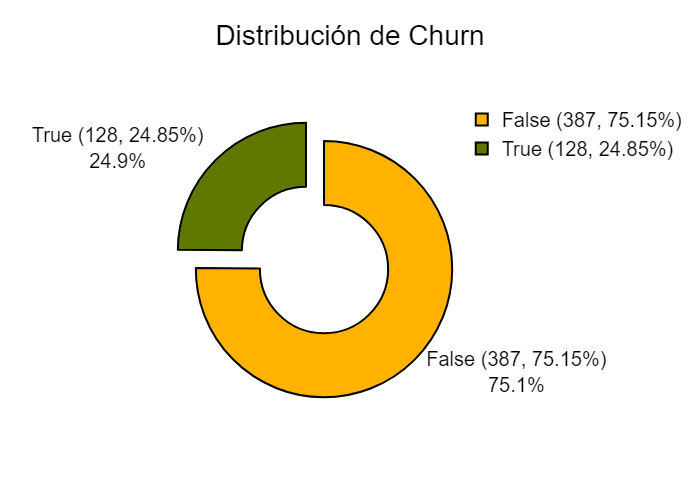
\includegraphics[scale=.45]{Gráficas e Imagenes/Distribucion_Churn.png}
		\caption{Gráfica de tarda para el abandono de clientes.}
		\label{fig:ChurnDistri}
	\end{figure}
\end{center}

En estas ultimas secciones he abordado a profundidad el concepto de \textit{churn}, el como analizar la actividad de compra de los clientes nos ayuda a comprender a como determinar el \textit{churn}, por lo cual en la siguiente sección realizaremos un tipo de análisis más enfocado al comportamiento histórico de los clientes y ver cual ha sido el \textit{churn} y retention rate.

\section{Análisis de Cohortes y la tasa de abandono}

Analizar el comportamiento del abandono de clientes a lo largo del tiempo nos puede ayudar a encontrar conductas que a simple vista suelen pasar desapercibidas. Por lo tanto cabe aclarar el significado de cohorte,  \citep{2020Gold} lo define como un grupo de individuos que son similares, y de hecho lo que nos interesa en este trabajo es estudiar esa similitud a lo largo del tiempo para poder encontrar patrones en el comportamiento del abandono de clientes. 

Por lo cual los grupos que definiremos serán periodos de tiempo, agruparemos aquellos clientes que tuvieron actividad durante dichos periodos, en particular para este trabajo definiremos los cohortes como meses, pero bien podrían ser semanas, años, etc. El objetivo de identificar estos cohortes es tener mayor claridad de la actividad mensual de los clientes y poder hacernos las siguiente preguntas. ¿Cuantos clientes activos tiene una empresa por mes? ¿Cuantos clientes nuevos han adquirido? y ¿Cuantos clientes han perdido?

Podemos estudiar el comportamiento de estos cohortes usando diferentes metricas, ya sea por el numero de suscripciones a un servicio, volumen de compra, valor de compra o numero de clientes activos, este ultimo es la que usaremos en este trabajo, ya que esto nos permitirá relacionarlo con un concepto previamente visto, el \textit{churn rate}.\footnote{Antes de continuar tenemos que aclarar que hay distintos tipos de enfoques para agrupar los clientes, estos enfoques son inherentes al negocio o empresa en el cual se quiera implementar, además esta fuertemente ligado a la información que tengamos disponible, por lo cual hay que tener en cuenta estas limitantes antes de llevar acabo el análisis de cohortes.} 

Hacer este análisis en python es tarea sencilla, primero es necesario tener la fecha de compra o fecha de facturación contenida en nuestro datafra, cabe aclarar que este ejercicio podría hacerse antes de determinar la variable de abandono, esto para evitar tener la correcta dimensión del dataframe con el que deseamos trabajar, ya que el nivel de detalle que deseamos tener para realizar este análisis es por fecha de compra, consumo, producto y clientes o usuarios. Aclarado lo anterior, podemos comenzar a revisar los pasos a seguir para hacer este análisis:


\textbf{Duda: ¿Sera mejor mostrar esto como pseudocódigo?}
\begin{enumerate}
	\item Ordenar las observaciones de nuestro dataframe por fecha y id de usuario.\footnote{Es necesario que la variable que contenga la fecha sea del tipo de datetime para poder obtener una salida correcta en este paso y en los posteriores.}
	\item Crear una variable que almacene el desplazamiento de cada cohorte en meses posteriores, esta variable nos ayuda a identificar los periodos de desplazamiento posterior a la adquisición de los clientes.
	\item Determinar el mes de adquisición del cohorte de clientes.
	\item Contar los clientes activos mensuales de cada cohorte y sus desplazamientos posteriores.
	\item Del conteo final hay que tomar los clientes iniciales de cada cohorte y dividir todos los conteos por el número de clientes iniciales.
\end{enumerate}

	
A continuación mostraremos la implementación de dicho análisis, el primero de los pasos esta ilustrado en el código \ref{CohortStep1}

\begin{lstlisting}[language=Python, caption=código del paso 1 del analisis de cohorte, label=CohortStep1]
	df.sort_values(by=['Fecha', 'bp_id'], inplace=True)
\end{lstlisting}

Y es que como bien lo indican las instrucciones simplemente tenemos que ordenar nuestro dataframe haciendo uso de la API de pandas. 

Ordenar los datos de esta manera nos asegura que los cohortes que creemos tengan coherencia cronológicamente, esto porque en el paso 2 y 3 para determinar el mes de adquisición del cohorte y los meses de desplazamiento nos basamos en los meses de actividad de los clientes, en el código \ref{CohortStep2} creamos la columna \textit{CohortMonth} la cual corresponde al mes de adquisición del cohorte, mientras que \textit{InvoiceMonth} es el mes de compra cada cliente.

\begin{lstlisting}[language=Python, caption=código del paso 2 del analisis de cohorte, label=CohortStep2]
	def get_month(x): return dt.datetime(x.year, x.month, 1)
	
	df['InvoiceMonth'] = df['Fecha'].apply(get_month)
	grouping = df.groupby('bp_id')['InvoiceMonth']
	df['CohortMonth'] = grouping.transform('min') 
\end{lstlisting}

De forma auxiliar y previo obtener el resultado final, necesitamos crear una función que extraiga los valores enteros de los campos  \textit{CohortMonth} y \textit{InvoiceMonth}, en el código \ref{CohortStep2.1} mostramos la definición de dicho método. 

\begin{lstlisting}[language=Python, caption=código para el método get\_date\_int, label=CohortStep2.1]
	def get_date_int(df, column):
		year = df[column].dt.year
		month = df[column].dt.month
		day = df[column].dt.day
		return year, month, day
\end{lstlisting}

Análogamente para mejorar la forma en que vemos la información obtenida en el paso 3 nos apoyamos de la función \textit{get\_date\_int}, el código \ref{CohortStep3.1} nos ayudará a crear una columna llamada CohortIndex, esta columna como su nombre es un conjunto de indices cuyo fin es representar los cohortes, osea nos permite tener una mejor visualización del desplazamiento de cada grupo de clientes.


\begin{lstlisting}[language=Python, caption=código para la obtención de la columna \textit{CohortIndex}, label=CohortStep3.1]
	invoice_year, invoice_month, _ = get_date_int(df, 'InvoiceMonth')
	cohort_year, cohort_month, _ = get_date_int(df, 'CohortMonth')
	years_diff = invoice_year - cohort_year
	months_diff = invoice_month - cohort_month
	df['CohortIndex'] = years_diff * 12 + months_diff + 1
\end{lstlisting}

Por otra parte, para obtener el paso 4 debemos hacer uso de una pivot table  agrupar los datos por \textit{CohortMonth} y \textit{CohortIndex}, así como agregar para obtener el resultado final, en el código \ref{CohortStep4} podemos observar como llevar acabo esta implementación. La utilidad de usar una tabla pivote para mostrar el resultado es porque gracias a esta forma podremos visualizar de mejor manera el desplazamiento desde el momento de adquisición para cada cohorte hasta la ultima actividad.

\begin{lstlisting}[language=Python, caption=código para la obtención de la columna \textit{CohortIndex}, label=CohortStep4]
	grouping = df.groupby(['CohortMonth', 'CohortIndex'])
	cohort_data = grouping['pd_id'].apply(pd.Series.nunique)
	cohort_data = cohort_data.reset_index()
	cohort_counts = cohort_data.pivot(index='CohortMonth',
	columns='CohortIndex',
	values='pd_id')
\end{lstlisting}

Finalmente para poder obtener la matriz de taza de retención tenemos que llevar acabo el paso 5, la implementación la mostraremos en fragmento de código \ref{CohortStep4} se crea la variable \textit{cohort\_sizes} que toma la primera columna, esta representa el número de clientes iniciales de cada cohorte, una vez hecho esto crearemos la tabla pivote final llamada \textit{retention}, la misma es resultado de dividir toda la pivot \textit{cohort\_counts} por \textit{cohort\_sizes}, tal y como se muestra en la ecuación \ref{EquationChurn}, de hecho ya podemos explicar el porque la ecuación del \textit{churn rate} considera el numero de clientes por periodos de tiempo, y es que esta es la mejor forma de analizar la tasa de retención.


\begin{lstlisting}[language=Python, caption=código para la obtención de la columna \textit{CohortIndex}, label=CohortStep5]
	\# Dependencias
	import seaborn as sns
	import matplotlib.pyplot as plt
	\# Calulo de la matriz de retencion
	cohort_sizes = cohort_counts.iloc[:,0]
	retention = cohort_counts.divide(cohort_sizes, axis=0)
	retention.round(3) * 100
	\# Visualizacion de matriz de retencion.
	plt.figure(figsize=(35, 30))
	plt.title('Retention rates')
	sns.heatmap(data = retention,
	yticklabels=df['CohortMonth'].sort_values().apply(lambda x: x.strftime("%Y %b, %d")).unique(),
	annot=True,
	linewidths=.2,
	fmt='.0%',
	cmap='coolwarm',
	vmin=0,
	vmax=1)
	plt.show()
\end{lstlisting}

La gráfica \ref{fig:CohortesCount} nos muestra el resultado final de las anteriores codificaciones, en los registros correspondientes a la primera columna podemos observar que la taza de retención es siempre del $100\%$ esto se debe a que son los clientes que tienen su primer actividad de compra dentro de ese cohorte, de tal forma que los registros de las columnas posteriores representan la actividad de los clientes después de su adquisición, por ejemplo, el cohorte enero de 2022 en el segundo mes\footnote{Ya que cada numero es una representación simplificada de cada cohorte, es importante tomar en cuenta que dicho numero se toma apartir del cohorte inicial, por ejemplo, para el cohorte enero de 2022 el numero 1 es igual al mismo mes, en cambio el numero 2 significa febrero de 2022, de forma similar el numero 3 es equivalente a marzo del 2022 y así sucesivamente hasta llegar al ultimo mes, por consecuencia ultimo mes solo tendrá datos hasta el indice 1, el penúltimo contiene información hasta el indice 2, etc.} (febrero de 2022) podemos observar una retención del $76\%$ de los clientes iniciales y para el ultimo indice podemos notar que se mantuvieron $64\%$ de los clientes que iniciaron en enero del 2022, esto quiere decir que en \textbf{Fecha final} se perdió el $36\%$ de los clientes ingresados en enero de 2022, esto dicho grupo de clientes tiene un comportamiento de compra habitual y guardan cierta fidelidad.


Similarmente, los clientes adquiridos en agosto de 2022 tienen un comportamiento similar hasta 6 meses después de la adquisición, sin embargo es a aparir del mes 7 que este comportamiento baja al $40\%$. El general la tasa de retención de clientes adquiridos en cada cohorte es bajo , ya que para el mes más reciente de cada cohorte podemos notar una baja tasa de retención, lo cual indica que la empresa ha perdido más clientes de los que ha ganado en los últimos meses.



%\begin{wrapfigure}{l}{0.25\textwidth}
	\begin{figure}[p]
		\vspace{-55mm}
		\hspace*{-5cm}
		\
		%\centering
		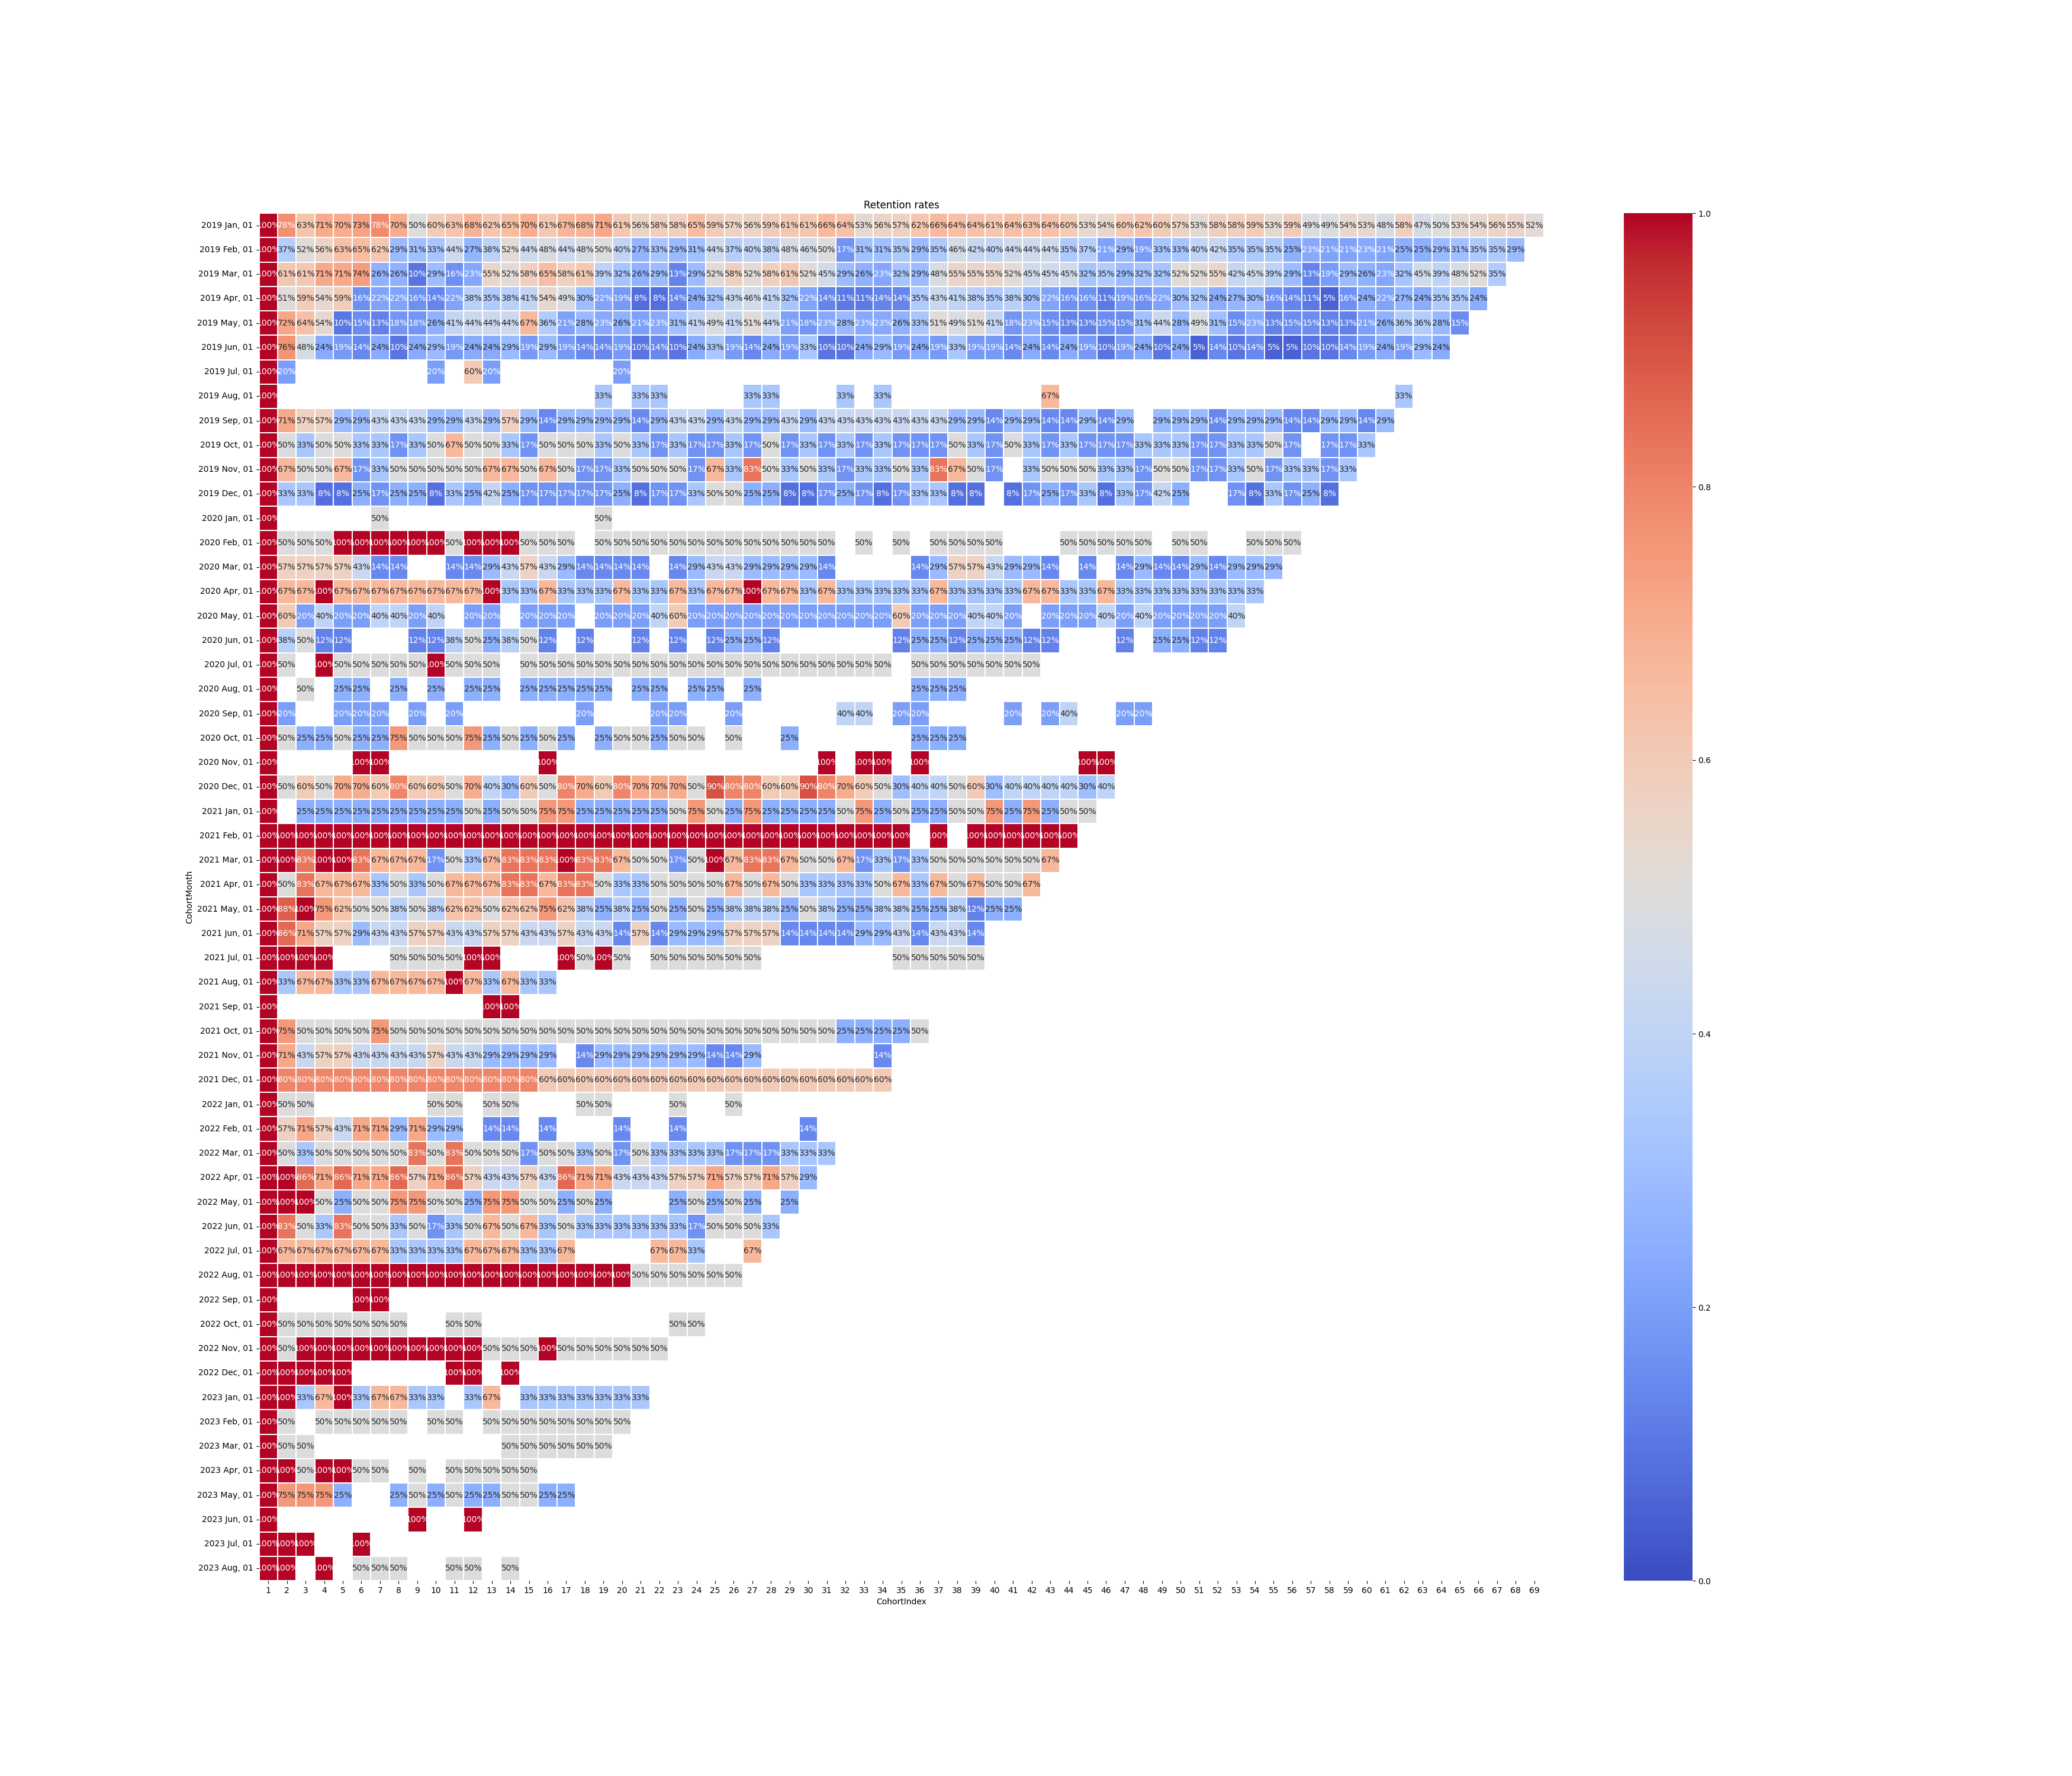
\includegraphics[scale=.3]{Gráficas e Imagenes/Cohort.png}
		\caption{Matriz de Cohortes.}
		\label{fig:CohortesCount}
	\end{figure}
%\end{wrapfigure}




\newpage
\section{Implementación de modelos de ML para predecir el abandono}

Una vez entendido el concepto de retención y abandono de clientes y las tasas y el análisis de cohorte, comenzaremos por mostrar la implementación de algoritmos de Machine Learning que nos permitan realizar predicciones del abandono. Recordemos que definimos la columna churn (abandono) como una variable de tipo binaria, donde true indica que un cliente abandono y false el caso contrario, en este caso nuestra variable objetivo sera la columna churn. 

En esta sección nos apoyaremos de las herramientas vistas en la sección 2 y más en especifico llevaremos acabo la implementación de modelos de clasificación binaria para poder predecir las etiquetas de la variable churn, por lo cual no profundizaremos mucho en la teoría detrás, sino nos enfocaremos unicamente en los resultados obtenidos y la interpretación de los mismos.

Para este trabajo compararemos los resultados de distintos modelos de clasificación binaria, tomando en cuenta las metricas de evaluación como precisión, exactitud, etc, haciendo uso tanto de herramientas visuales y resúmenes estadísticos veremos las desventajas y ventajas de cada modelo, esto eventualmente nos conducirá a determinar el modelo que mejor realice la clasificación.


Antes de empezar con el análisis comparativo, es conveniente aclarar que los modelos que en adelante analizaremos ya fueron optimizados y entrenados en el capitulo anterior, por lo cual en esta sección tomaremos como punto de partida lo visto en el capitulo anterior. 
% Duda sobre esta sección.

\subsection{Evaluación del modelo.}

Previo a la profundización en cada modelo y sus resultados veremos como evaluar el rendimiento de cada modelo, en esta sección utilizaremos como ejemplo el modelo de regresión logística, por lo cual lo visto de aquí en adelante es fácilmente reproducible a cualquier otro modelo. Partiremos de las predicciones con el conjunto de datos de validación, así nos apoyaremos de la matriz de confusión y curva roc para evaluar nuestros modelos de forma visual y numérica.

\begin{figure}[h]
	%\vspace{-55mm}
	%\hspace*{-5cm}
	\centering
	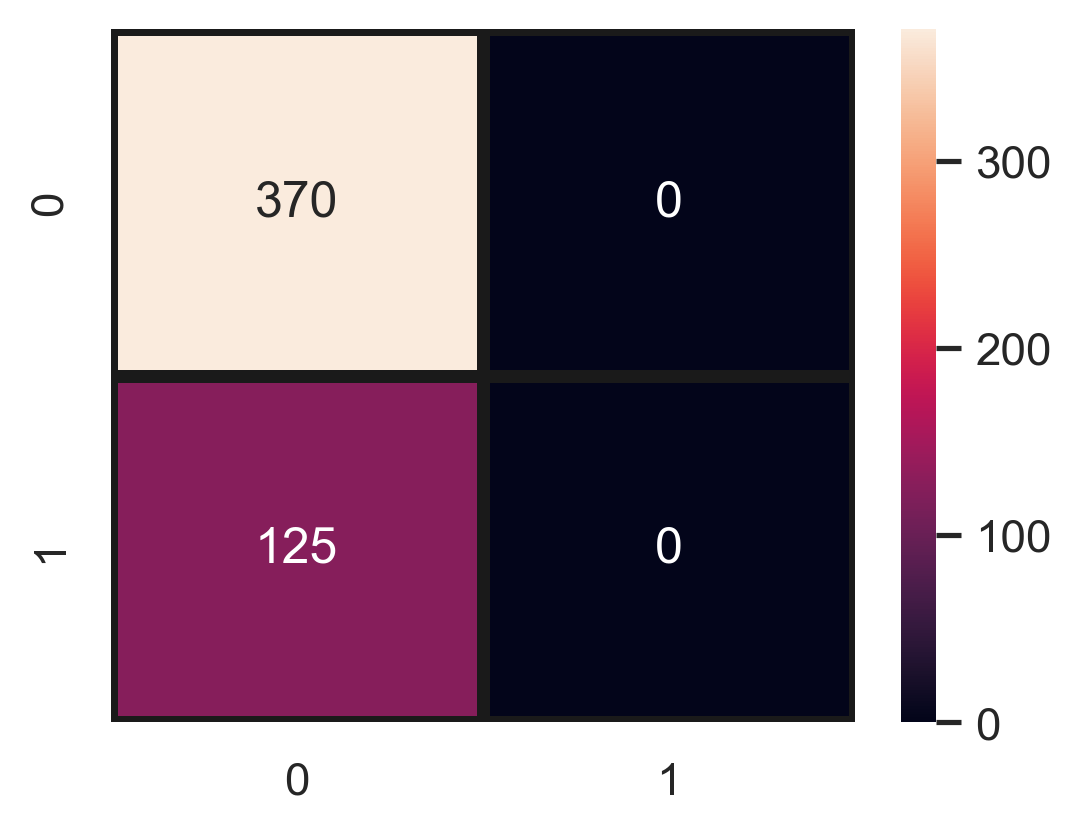
\includegraphics[scale=.4]{Gráficas e Imagenes/Confusion_matrix_train.png}
	\caption{Matriz de confusión para el modelo de regresión logística.}
	\label{fig:MatrizConfusion}
\end{figure}

En la gráfica \ref{fig:MatrizConfusion} podemos apreciar el numero de aciertos (verdaderos positivos y negativos) y el numero de errores (falsos positivos y negativos) cometidos por el modelo. La representación gráfica anteriormente mencionada es la matriz de confusión asociada al modelo de regresión logística, de hecho esta gráfica nos permite encontrar la mayoría de las metricas para evaluar nuestro modelo. Por ejemplo, la ecuación \ref{EquationAcurracy}\footnote{Las variables TP, TN,FP y FN son el numero de casos true positives, true negatives, false positives y false negatives respectivamente.} nos proporciona la \textit{accuracy} o exactitud, esta métrica nos indica el porcentaje de acierto que tuvo el modelo. Python nos facilita el calculo de esta métrica, el código \ref{pymetrics} muestra un ejemplo de como calcular la accuracy haciendo uso del sklearn.

\textbf{Aquí pienso colocar el análisis de la matriz de este modelo, decidí no añadirlo por que puede cambiar.}

\begin{equation}
	\textrm{accuracy}=\frac{TP+TN}{(TP+TN+FP+FN)} 
	\label{EquationAcurracy}
\end{equation}

Sin embargo \citet{2023Peterson} menciona que la accuracy usualmente no es una buena métrica para evaluar modelos cuando tenemos clases desbalanceadas en nuestra variable objetivo, lo cual es nuestro caso, ya que como mencionamos anteriormente la variable \textit{churn} tiene más registros marcados como \textit{false}, aun que en el capitulo anterior explicamos la forma en que lidiamos con el desbalance de las clases, explicaremos por que no siempre es conveniente optar por la exactitud, esto porque puede encubrir un incorrecto funcionamiento del modelo, por ejemplo, la matriz \ref{fig:MatrizConfusion} podemos notar que el total de las observaciones que inicialmente fueron clasificadas como false son mayores a las clasificados como true, el problema es que aunque el porcentaje de aciertos en la clase con dominante es medianamente aceptable, siento mayor a $90\%$, la clase minoritaria muestra un menor rendimiento, \textbf{insertar porcentaje} esta cifra indica el mal rendimiento para los registros clasificados como true.

Y es que aun que la clase true sea minoritaria, nos interesa tener la mayor cantidad de predicciones correctas para que en un futuro poder predecir correctamente los clientes que están abandonaran la compañía. Por lo tanto recomendamos optar por otras metricas para tener una visión mas completa del rendimiento de nuestro modelo. 

\begin{lstlisting}[language=Python, caption=código para calculo de metricas, label=pymetrics]
	from sklearn.metrics import accuracy_score,confusion_matrix, classification_report, precision_score, recall_score, f1_score
	print("Accuracy: {}".format(accuracy_score(y_true=valid['y'],y_pred=valid['y^_lr'])))
	print("Precision: {}".format(precision_score(y_true=valid['y'],y_pred=valid['y^_lr'])))
	print("Recall: {}".format(recall_score(y_true=valid['y'],y_pred=valid['y^_lr'])))
	print("F1: {}".format(f1_score(y_true=valid['y'],y_pred=valid['y^_lr'])))
\end{lstlisting}

Algunas de las metricas a las que podemos recurrir son precision (precisión), recall (sensibilidad o recuperación) y $F_\beta$. Aun que existe muchas otras metricas, nosotros nos enfocaremos solo en estas. La precisión (ecuación \ref{Equationprecision}) es el número de aciertos, predicciones correctas, entre el total de casos positivos captados por el modelo, osea del total de casos clasificados como true, cuales son realmente true, mientras que la sensibilidad (ecuación \ref{EquationRecall}) es el numero de predicciones correctas, entre el total de casos positivos, es decir es la proporción de casos clasificados como true.

\begin{equation}
	\textrm{precision}=\frac{TP}{(TP+FP)} 
	\label{Equationprecision}
\end{equation}

\begin{equation}
	\textrm{recall}=\frac{TP}{(TP+FN)} 
	\label{EquationRecall}
\end{equation}

Hay distintas ventajas de usar una u otra métrica para evaluar nuestro modelo, si nosotros decidimos inclinarnos por la recall, estaríamos dando mayor importancia a reducir la cantidad de errores cometidos por el modelo, esto nos indica que esta métrica no nos aporta información acerca de los falsos positivos, y lo mismo pasa con la presicion, ya que al querer reducir el numero de falsos positivos estaríamos ignorando el rendimiento del modelo frente los falsos negativos, por lo cual escoger una u otra es decisión del científico de datos a cargo, en el código \ref{pymetrics} nos muestra como calcular estas dos metricas con ayuda de Python.

\begin{equation}
	F_\beta=(1+\beta^2)\cdot \frac{\textrm{precision}\cdot \textrm{recall}}{\beta^2\cdot(\textrm{precision}+\textrm{recall})} 
	\label{EquationFB}
\end{equation}

La métrica que nos permite encontrar un equilibrio entre el numero de FP y FN es el F-score, esta métrica combina tanto la precision y recall en un solo valor, la ecuación \ref{EquationFB} nos permite calcular dicho valor. El parámetro de $\beta$ nos da la posibilidad de otorgarle un nivel de importancia a la precision o recall. De hecho si el valor de $\beta$ es igual a cero el F-score le da mayor importancia a la precision, mientras que cuando $\beta$ es igual a 0.5 el $F-score$ le da mayor peso a la recall, por ultimo si $\beta$ es igual a 1, obtenemos el $F_1$-score (ecuación \ref{EquationF1}) le damos igual importancia a ambas metricas, de esta forma podemos evaluar tanto el número de falsos positivos y negativos.


\begin{equation}
	F_1=2\cdot \frac{\textrm{precision}\cdot \textrm{recall}}{(\textrm{precision}+\textrm{recall})} 
	\label{EquationF1}
\end{equation}


De la comparación entre precision y recall, surge otra forma de evaluar modelos de clasificación binaria, esta métrica es la curva roc (Receiver Operating Characteristic), \citet[p. 91]{2017Géron} nos dice que \textit{la curva ROC representa gráficamente la tasa de verdaderos positivos frente a la tasa de falsos positivos. La FPR es la proporción de casos negativos que se clasifican incorrectamente como positivos.} 

\begin{figure}[h]
	%\vspace{-55mm}
	%\hspace*{-5cm}
	\centering
	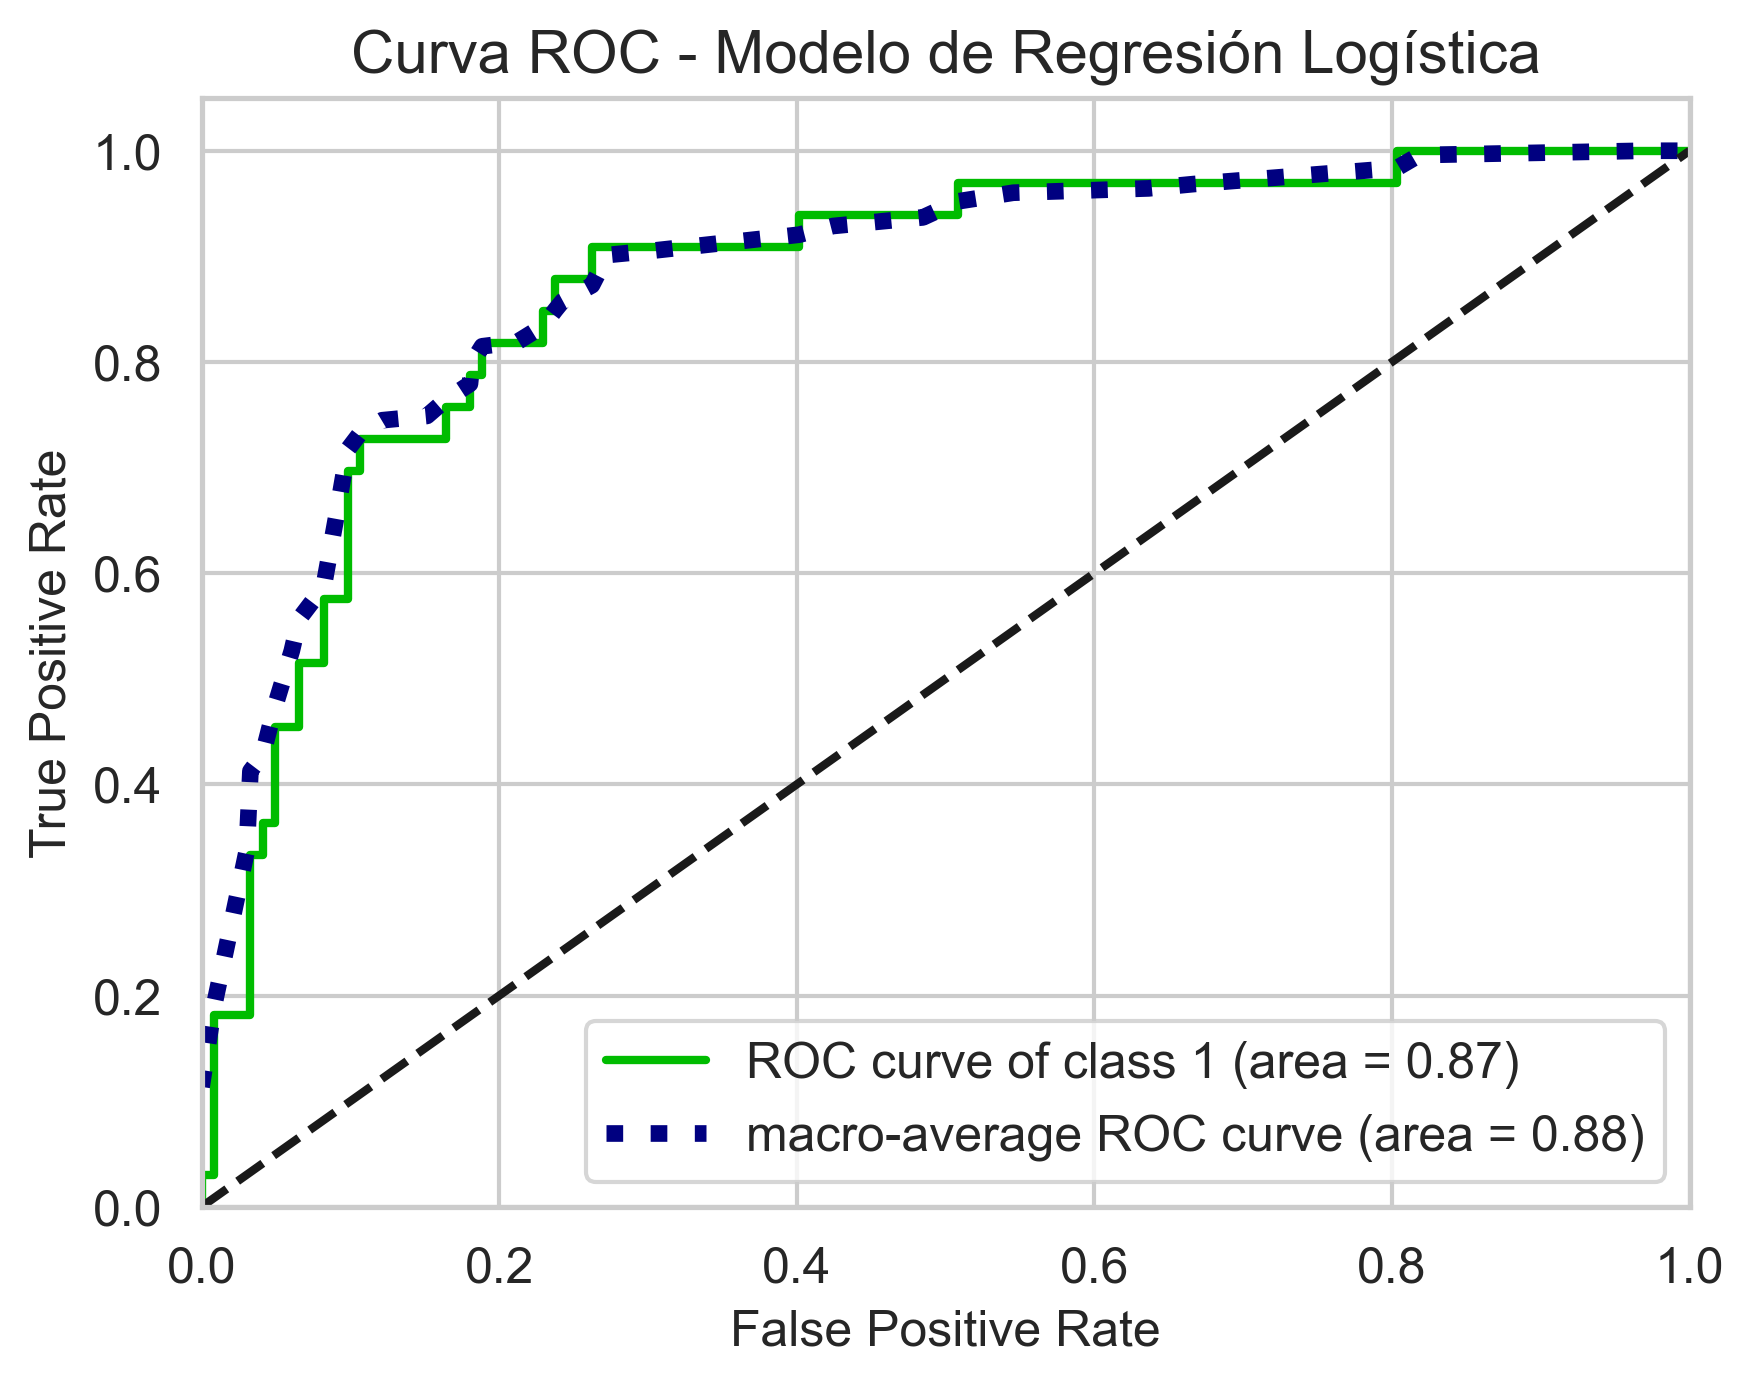
\includegraphics[scale=.6]{Gráficas e Imagenes/curva_roc_logistica_valid.png}
	\caption{Curva ROC.}
	\label{fig:CurvaRoc}
\end{figure}

En la gráfica \ref{fig:CurvaRoc} podemos notar que el eje de ordenas esta etiquetado como True Positive Rate (TPR), mientras que el eje de abscisas esta etiquetado como False Positive Rate (FPR), donde las TPR puede ser también interpretado como la recall mientras que FPR suele interpretarse como el complemento de la especificidad (1- especificidad), \citep{2017Géron} menciona que un buen clasificador se mantiene lo más posible alejado de la linea vertical punteada, dicha linea diagonal sirve más como una referencia y es también es llamada línea de no-discriminación.

Además de la curva roc, el área bajo la curva roc (comúnmente llamada AUC) es otra muy buena opción para medir el rendimiento de modelos de clasificación binaria, ya que un valor cercano a 1 de la AUC nos indicara que el contamos con un buen clasificador, este buen rendimiento se considera respecto a la especificidad y recall, es decir, estas dos metricas nos indica que nuestro modelo en cuestión dará una mejor calificación a la probabilidad de un registro positivo seleccionado al azar que a un registro negativo seleccionado de forma aleatoria.

De hecho este ultimo punto deja en evidencia que existe cierto inconveniente al evaluar nuestros modelos con la auc solamente, ya que la curva roc puede encubrir desbalances entre clases de la variable objetivo, \cite{Chugh2023} plantea que la curva roc tiende a pasar por alto el desequilibrio entre clases, ya que la tasa de FP es una métrica que solo contempla a la clase negativa, lo que significa que se espera que el cambio en FP sea proporcional al cambio en FP+TN (todos los casos negativos), esto puede derivar en tener poca sensibilidad a cambios en la distribución de las clases de la variable objetivo.

Partiendo de este ultimo punto y recordando que en nuestro caso la información que estamos analizando tiene cierto desequilibrio entre clases de la variable a predecir, sin embargo no todo esta perdido, ya que existe otra métrica que nos proporciona mayor información que la auc y que no pasa por alto el desequilibrio en entre clases, esta métrica es la curva precision-recall, en palabras de \citet{Chugh2023} \textit{una curva ROC es similar a la curva PR (Precision Recall), pero traza la tasa de verdaderos positivos (TPR) frente a la tasa de falsos positivos (FPR) para diferentes umbrales... La PR es comparativamente más informativa. Esto se debe a que la curva P-R proporciona información más significativa sobre la clase de interés en comparación con la curva ROC.} 


\begin{figure}[h]
	%\vspace{-55mm}
	%\hspace*{-5cm}
	\centering
	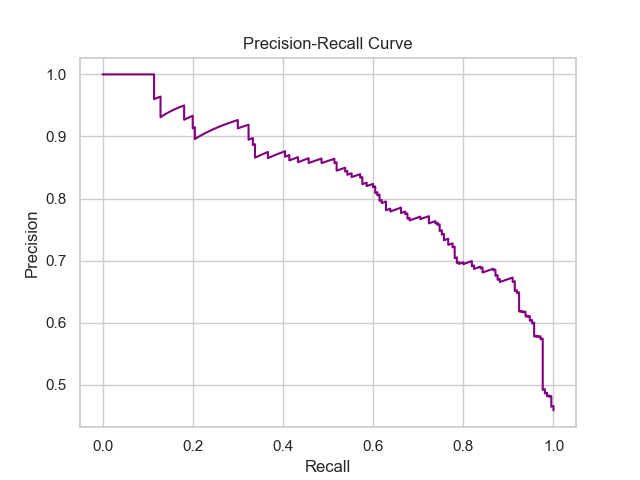
\includegraphics[scale=.6]{Gráficas e Imagenes/precision_recall_curve.png}
	\caption{Curva PR.}
	\label{fig:CurvaPR}
\end{figure}

Por lo tanto la curva PR nos ayudara a evaluar de mejor manera nuestros datos dando mayor importancia a los registros positivos pero sin dejar completamente de lado los negativos, encontrando así un equilibrio no arbitrario entre uno y otro. Esto porque uno de los grandes inconvenientes de elegir la auc sobre la PR es que en nuestro caso al tener mayor proporción de registros clasificados negativamente (osea como no abandono) hace que la tasa de FP sea demasiado pequeña, en comparación de la PR que al considerar la a la precision y por ende el rendimiento de nuestro modelo en los registros positivos.

\subsection{Comparación del rendimiento entre modelos.}

%DataCamp. (Año). Marketing Analytics: Predicting Customer Churn in Python. Recuperado de DataCamp.
